\documentclass[a4j]{jarticle}

\usepackage[dvipdfmx]{graphicx}

\title{基本句・内容語の説明書}
\author{河原 大輔 \and 黒橋 禎夫}
\date{2008年8月5日}

\newcommand{\sm}[1]{\textless #1\textgreater}

\begin{document}
\maketitle

\section{基本句}

基本句は格・省略解析などにおける処理の基本単位である。形態素を以下のよう
に分類する。基本句は、内容語1つを核とする形態素列である。ただし、英語の
句の場合のみ、1基本句内に内容語が複数存在する。

% \begin{quote}
%      例) 河野洋平, 
%          マイケル・フェイ君, 
%          ジョン・F・ケネディ
% \end{quote}

\begin{figure}[h]
 \begin{center}
  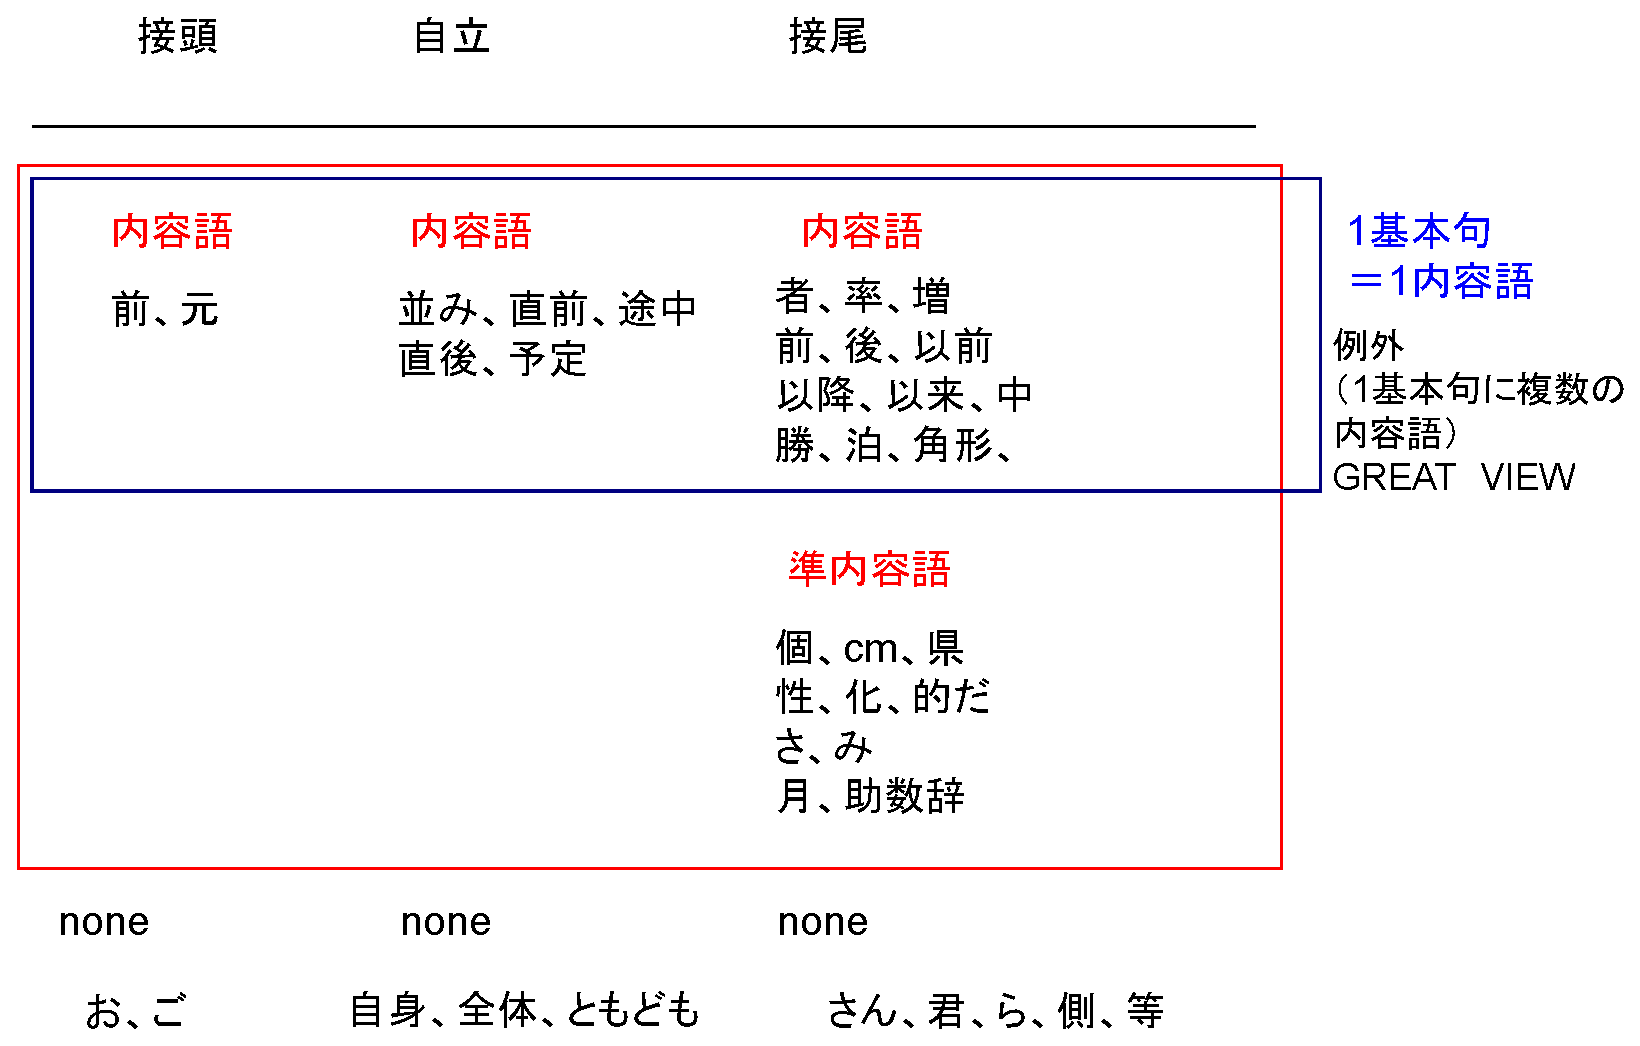
\includegraphics[scale=0.50]{bp.eps}
 \end{center}
\end{figure}

% \begin{tabular}{llll} \cline{1-3}
% \sm{内容語}の接頭辞       & \sm{自立} & \sm{内容語}の接尾辞   & $\leftarrow$独立語かつ内容語 \\ \cline{1-3}
%                           &           & \sm{準内容語}の接尾辞 & $\leftarrow$内容語 \\ \cline{1-3}
% \sm{内容語}ではない接頭辞 &           & \sm{内容語}\sm{準内容語}ではない接尾辞 & \\
%                           &           & その他(助詞, 助動詞, 特殊, ...) \\ \cline{1-3}
% \end{tabular}
% \hspace*{4mm} {\small ※ KNPのfeatureになっているものに\sm{}を付与している。}

% \vspace*{3ex}


\section{内容語・準内容語}

\sm{内容語}や\sm{準内容語}とは、意味属性を取得したり、キーワードとして用
いるべき形態素である。\sm{準内容語}は、基本句として独立しないが、何かし
らの意味を保持する接尾辞である。


※ 従来は\sm{意味有}というfeatureであったが、\sm{内容語}または\sm{準内容
語}に改名された。


\section{独立語、内容語の観点からの接頭・接尾辞の分類}
\label{Section::PrefixSuffix}

以下のように、接頭辞は2つ、接尾辞は3つに分かれる。
\begin{itemize}
 \item 接頭辞
       \begin{itemize}
	\item \sm{内容語}
	\item それ以外
       \end{itemize}
 \item 接尾辞
       \begin{itemize}
	\item \sm{内容語}
	\item \sm{準内容語}
	\item それ以外
       \end{itemize}
\end{itemize}
% \sm{準内容語}は\sm{内容語}に似ているが、基本句として独立しない接尾辞である。

\vspace*{2ex}

以下に、それぞれに属する形態素リストを示す。

\begin{itemize}
 \item 接頭辞
       \begin{itemize}
	\item \sm{内容語}
	      \begin{itemize}
	       \item 名詞接頭辞
		     \begin{quote}
		      再 準 新 旧 超 高 低 猛 全 現 前 元 故 好 長 短 諸 被 真 真っ 真ん 大 中 小 両 本 同 各 今 来 最 他 初 副 名 昨 毎 翌 実 主 総 プレ
		     \end{quote}
	      \end{itemize}
	\item 非内容語

	      \begin{itemize}
	       \item 名詞接頭辞
		     \begin{quote}
		      御 お み す 第 約 まる ひと
		     \end{quote}

	       \item 動詞接頭辞、イ形容詞接頭辞、ナ形容詞接頭辞のすべて
	      \end{itemize}
       \end{itemize}
 \item 接尾辞
       \begin{itemize}
	\item \sm{内容語}
	      \begin{itemize}
	       \item 名詞性名詞助数辞
		     \begin{quote}
		      社 会 条 項 単位 種類 連続 余り 戦 勝 敗 泊 角形
		     \end{quote}
	       \item 名詞性特殊接尾辞
		     \begin{quote}
		      増 減 暮れ 末 以前 以後 以来 以降
		     \end{quote}
	       \item 名詞性名詞接尾辞
		     \begin{quote}
		      前 中 後 前後 率 通り 型 形 用 製 家 者 数 代 費 学 向き 向け 入り 明け \\ 作り 造り づくり ずみ 無し なし 行き 宛 あて どころ
		     \end{quote}
	       \item 名詞性述語接尾辞
		     \begin{quote}
		      方 手 放題
		     \end{quote}
     	      \end{itemize}
	\item \sm{準内容語}
	      \begin{itemize}
	       \item 名詞性名詞助数辞のうち\sm{内容語}でないもの
	       \item 名詞性特殊接尾辞
		     \begin{quote}
		      都 道 府 県 郡 市 村 町 区 州 省
		     \end{quote}
     	       \item 名詞性名詞接尾辞
		     \begin{quote}
		      性 化 以外
		     \end{quote}
	       \item 名詞性述語接尾辞
		     \begin{quote}
		      さ 味 み
		     \end{quote}
     	       \item 形容詞性名詞接尾辞
		     \begin{quote}
		      的だ がちだ 気味だ
		     \end{quote}
	       \item 形容詞性述語接尾辞
		     \begin{quote}
		      目だ めだ 気だ げだ
		     \end{quote}
     	      \end{itemize}
	\item 非内容語
	      \begin{itemize}
	       \item 名詞性特殊接尾辞
		     \begin{quote}
		      超 以内 限り 過ぎ 半 強 弱 付
		     \end{quote}
	       \item 名詞性名詞接尾辞
		     \begin{quote}
		      さん 君 様 殿 氏 ちゃん 以上 以下 未満 近く くらい ぐらい 等 程 間 程度 \\ 頃 ごろ ずつ 当たり 辺り おき 毎 振り 振 ぶり っぷり 目 だらけ さなか \\ かたがた 自体 達 ら 同士 ども 方 勢 っ子 調 上 下 そのもの がかり \\ 足らず たらず がらみ ぐるみ ならでは ぞろい がえ 側 ずくめ 尽くし \\ つくし ずく ごとき 如き 内 その他 級 づたい 別
		     \end{quote}
	       \item 名詞性述語接尾辞
		     \begin{quote}
		      たて 振り 振 ぶり っぷり 様 がい っこ
		     \end{quote}
	       \item 形容詞性名詞接尾辞
		     \begin{quote}
		      くさい っぽい い
		     \end{quote}
     	       \item 形容詞性述語接尾辞
		     \begin{quote}
		      ない たい やすい よい にくい がたい 難い づらい がちだ そうだ
		     \end{quote}
	       \item 動詞性接尾辞のすべて
	      \end{itemize}
       \end{itemize}
\end{itemize}


% \section{代表表記}

%        \begin{itemize}
% 	\item JUMANで以下の形態素に付与

% 	      名詞(普通, サ変, 副詞的), 動詞, 形容詞, 副詞, 連体詞, 接続
% 	      詞, 感動詞, 接頭辞, 接尾辞

% 	\item KNPで疑似代表表記を付与

% 	      名詞(形式, 人名, 地名, 組織名, 固有, 数詞), 連語, 未知語

% 	\item 付与しないもの

% 	      助詞, 助動詞, 判定詞, 特殊
%        \end{itemize}


% \subsection{疑似代表表記}

%        \begin{itemize}
% 	\item 疑似代表表記のフォーマット

% 	      \begin{itemize}
% 	       \item 代表表記を、形態素の原形、形態素の読みから、``代表
% 		     表記:(形態素の原形)/(形態素の読み)''という形式で作
% 		     成し、形態素解析結果列の12番目、および、\sm{}で囲まれ
% 		     て出力される素性に追加

% 	       \item 疑似代表表記であることを示すために、\sm{疑似代表表記}
% 		     という素性を付与

% 		     例:"疑似代表表記 代表表記:マッキントッシュ/マッキントッシュ"

% 		     \sm{疑似代表表記}\sm{代表表記:マッキントッシュ/マッキントッシュ}

% 	       \item 疑似代表表記を付与した語に曖昧性がある場合は、ALT素性にもその情報を記述

% 		     例:\sm{ALT-秋田-あきた-秋田-6-4-0-0-"疑似代表表記 代表表記:秋田/あきた"}
% 	      \end{itemize}
%        \end{itemize}


% \subsection{正規化代表表記}

% さまざまなアプリケーションで使用するために、形態素、基本句、文節のそれぞ
% れに対して付与している。曖昧性を保持し、複合名詞なら代表表記を連結してい
% る。


% \subsubsection{形態素}

% 代表表記(疑似代表表記を含む)をもつ形態素に付与

%  \begin{tabular}{ll@{ $\leftarrow$ }l}
%   例) & 大学 & \sm{正規化代表表記:大学/だいがく} \\
%       & 湖   & \sm{正規化代表表記:湖/こ?湖/みずうみ} \\
%       & なる & \sm{正規化代表表記:成る/なる?鳴る/なる} \\
%  \end{tabular}


% \subsubsection{基本句}

% 基本句内の内容語の正規化代表表記を結合

%  \begin{tabular}{ll@{ $\leftarrow$ }l}
%   例) & 大学に & \sm{正規化代表表記:大学/だいがく} \\
%       & 湖に & \sm{正規化代表表記:湖/こ?湖/みずうみ} \\
%       & 東京都に & \sm{正規化代表表記:東京/とうきょう+都/と} \\
%       & はやさに & \sm{正規化代表表記:早い/はやい?速い/はやい+さ/さ} \\
%  \end{tabular}


% \subsubsection{文節}

% 文節内の基本句の正規化代表表記の結合 = 文節内の内容語の正規化代表表記の結合

%  \begin{tabular}{ll@{ $\leftarrow$ }l}
%   例) & 京都大学に & \sm{正規化代表表記:京都/きょうと+大学/だいがく} \\
%       & アジア・太平洋経済協力会議の & \sm{正規化代表表記:アジア/あじあ+太平洋/たいへいよう+経済/けいざい+協力/きょうりょく+会議/かいぎ} \\
%       & 計算機を & \sm{正規化代表表記:計算/けいさん+機/き} \\
% \end{tabular}

% \vspace*{2ex}

% また、文節内最後の基本句の正規化代表表記を\sm{主辞代表表記:...}で付与。

%  \begin{tabular}{ll@{ $\leftarrow$ }l}
%   例) & 京都大学に & \sm{主辞代表表記:大学/だいがく} \\
%       & アジア・太平洋経済協力会議の & \sm{主辞代表表記:会議/かいぎ} \\
%       & 計算機を & \sm{主辞代表表記:機/き} \\
%  \end{tabular}

% \vspace*{2ex}

% さらに、文節内最後の内容語が一文字漢字の場合は、文節内最後の2内容語の正規化代表表記を結合し\sm{主辞’代表表記:...}で付与。

%  \begin{tabular}{ll@{ $\leftarrow$ }l}
%   例) & 計算機を & \sm{主辞’代表表記:計算/けいさん+機/き} \\
%  \end{tabular}

% \noindent
% ※ これを\sm{主辞代表表記:...}にする予定


\section{問題}

\begin{itemize}
 \item 一つの基本句に複数の\sm{内容語}(または\sm{準内容語})がある場合に検索で問題発生

       \begin{itemize}
% 	\item 複数の\sm{内容語}
%
% 	      例) 河野洋平

	\item \sm{内容語}+\sm{準内容語}

	      例) 3個, 3冊, 東京都, 可能性, 国際化, 長さ, 積極的だ
       \end{itemize}

       $\rightarrow$ 検索側で対処

%  \item あまり意味のない代表表記の曖昧性

%        \begin{itemize}
% 	\item 人名、地名などの読みの曖昧性
% 	\item 音訓
%        \end{itemize}

%        $\rightarrow$ 代表表記は統一方向へ (音訓は音の代表表記)


%  \item 代表表記のIDとしての一意性

%        例) 清水 $\leftarrow$ 清水/しみず (普通名詞), 清水/しみず (地名), 清水/きよみず (地名)

%        $\rightarrow$ 代表表記に品詞細分類の記号を付与する予定

\end{itemize}


\end{document}
